% $HeadURL$

To set the stage for what follows in this chapter, we first give a brief overview of some of the concepts in the \PD notation with the help of an example shown in \fig{eg1}.

\begin{figure}[H]
  \centering
  \vspace*{-0.75em}
  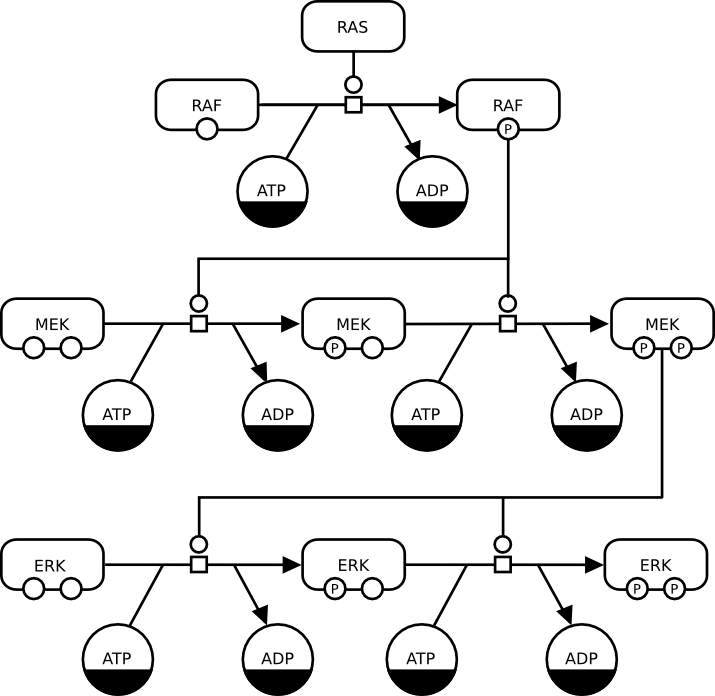
\includegraphics[scale=0.8]{examples/MAPK-only}
  \caption{This example of a \PD uses two kinds of entity pool nodes: one
    for pools of different macromolecules (\sect{macromolecule}) and
    another for pools of simple chemicals (\sect{simpleChemical}).  Most
    macromolecule nodes in this map are adorned with state
    variables (\sect{stateVariable}) representing phosphorylation states.
    This map uses one type of process node, the process node
    (\sect{process}), and one kind of connecting arc, catalysis
    (\sect{catalysis}).  Finally, some entity pool nodes have dark bands
    along their bottoms; these are clone markers indicating that the same
    pool nodes appear multiple times in the map.}
  \label{fig:eg1}
\end{figure}

The map in \fig{eg1} is a simple map for part of a mitogen-activated protein kinase (MAPK) cascade.  The larger nodes in the figure (some of which are in the shape of rounded rectangles and others in the shape of circles) represent biological materials---things like macromolecules and simple chemicals.  The biological materials are altered via processes, which are indicated in \PD by lines with arrows and other decorations.  In this particular map, all of the processes happen to be the same: processes catalyzed by biochemical entities.  The directions of the arrows indicate the direction of the processes; for example, unphosphorylated RAF kinase processes to phosphorylated RAF kinase via a process catalyzed by RAS. Although ATP and ADP are shown as incidental to the phosphorylations on this particular graph, they are involved in the same process as the proteins getting phosphorylated. The small circles on the nodes for RAF and other entity pools represent state variables (in this case, phosphorylation sites). 

The essence of the \PD is \emph{change}: it shows how different entities in the system process from one form to another.  The entities themselves can be many different things.  In the example of \fig{eg1}, they are either pools of macromolecules or pools of simple chemicals, but as will become clear later in this chapter, they can be other conceptual and material constructs as well.  Note also that we speak of \emph{entity pools} rather than individuals; this is because in biochemical network models, one does not focus on single molecules, but rather collections of molecules of the same kind.  The molecules in a given pool are considered indistinguishable from each other.  The way in which one type of entity is transformed into another is conveyed by a \emph{process node} and links between entity pool nodes and process nodes indicate an influence by the entities on the processes.  In the case of \fig{eg1}, those links describe consumption \sect{consumption}, production \sect{production} and catalysis \sect{catalysis}, but others are possible.  Finally, nodes in \PDs are usually not repeated; if they do need to be repeated, they are marked with \emph{clone markers}---specific modifications to the appearance of the node (\sect{cloneMarker}). The details of this and other aspects of \PD notation are explained in the rest of this chapter.

\tab{component-summary} summarizes the different SBGN abstractions described in this chapter.

\newcolumntype{P}[1]{>{\raggedright\hspace{0pt}\arraybackslash}p{#1}}

\begin{table}[bh]
  \centering
  \small
  \begin{tabular}{@{}llP{2.4in}P{1.6in}@{}}
    \toprule
    \textbf{Component} & \textbf{Abbrev.} & \textbf{Role} & \textbf{Examples}\\
    \midrule
    Entity pool node
    & EPN
    & A population of entities that cannot be distinguished from each other
    & Specific macromolecules or other chemical species \\[0.5em]

    Container node	
    & CN
    & An encapsulation of one or more other SBGN constructs
    & Complexes, compartments \\[1.6em]

    Process node
    & PN
    & A process that transforms one or more EPNs into one or more other EPNs
    & Process, association, dissociation \\[0.5em]

    Arc
    & ---
    & Links between EPNs or CNs to PNs or CNs to indicate influences
    & Production, catalysis, inhibition \\[0.5em]

    Logical operators
    & ---
    & Combines one or several inputs into one output
    & Boolean \emph{and}, \emph{or}, \emph{not} \\
    \bottomrule
  \end{tabular}
  \caption{Summary of \PD components and their roles.}
  \label{tab:component-summary}
\end{table}






%%% Local Variables: 
%%% mode: latex
%%% TeX-master: "../sbgn_PD-level1"
%%% End: 
